% This is "sig-alternate.tex" V2.1 April 2013
% This file should be compiled with V2.5 of "sig-alternate.cls" May 2012
%
% This example file demonstrates the use of the 'sig-alternate.cls'
% V2.5 LaTeX2e document class file. It is for those submitting
% articles to ACM Conference Proceedings WHO DO NOT WISH TO
% STRICTLY ADHERE TO THE SIGS (PUBS-BOARD-ENDORSED) STYLE.
% The 'sig-alternate.cls' file will produce a similar-looking,
% albeit, 'tighter' paper resulting in, invariably, fewer pages.
%
% ----------------------------------------------------------------------------------------------------------------
% This .tex file (and associated .cls V2.5) produces:
%       1) The Permission Statement
%       2) The Conference (location) Info information
%       3) The Copyright Line with ACM data
%       4) NO page numbers
%
% as against the acm_proc_article-sp.cls file which
% DOES NOT produce 1) thru' 3) above.
%
% Using 'sig-alternate.cls' you have control, however, from within
% the source .tex file, over both the CopyrightYear
% (defaulted to 200X) and the ACM Copyright Data
% (defaulted to X-XXXXX-XX-X/XX/XX).
% e.g.
% \CopyrightYear{2007} will cause 2007 to appear in the copyright line.
% \crdata{0-12345-67-8/90/12} will cause 0-12345-67-8/90/12 to appear in the copyright line.
%
% ---------------------------------------------------------------------------------------------------------------
% This .tex source is an example which *does* use
% the .bib file (from which the .bbl file % is produced).
% REMEMBER HOWEVER: After having produced the .bbl file,
% and prior to final submission, you *NEED* to 'insert'
% your .bbl file into your source .tex file so as to provide
% ONE 'self-contained' source file.
%
% ================= IF YOU HAVE QUESTIONS =======================
% Questions regarding the SIGS styles, SIGS policies and
% procedures, Conferences etc. should be sent to
% Adrienne Griscti (griscti@acm.org)
%
% Technical questions _only_ to
% Gerald Murray (murray@hq.acm.org)
% ===============================================================
%
% For tracking purposes - this is V2.0 - May 2012

\documentclass{sig-alternate-05-2015}
\usepackage{color} %je jen na cervenou barvu  -  oddelat nakonec
\usepackage{booktabs} 
\usepackage{algorithm2e}
\usepackage{amsmath}
\usepackage{amssymb}
\usepackage{url}
%\usepackage{subfig}

\usepackage{subcaption}
\usepackage{cleveref}
\usepackage{graphicx}
\newtheorem{example}{Example}
%\theoremstyle{definition}
%\newtheorem{definition}{Definition}
\newdef{definition}{Definition}
\newtheorem{remark}{Remark}

%code to remove doi: http://tex.stackexchange.com/questions/301482/acm-sig-template-unwanted-acm-isbn-and-doi
\makeatletter
\def\@copyrightspace{\relax}
\makeatother

\begin{document}

% Copyright
%\setcopyright{acmcopyright} 

\title{Around Average Behavior: 3-lambda Network Model} %Data Sampling Based on Representatives

\numberofauthors{3}
\author{
% You can go ahead and credit any number of authors here,
% e.g. one 'row of three' or two rows (consisting of one row of three
% and a second row of one, two or three).
%
% The command \alignauthor (no curly braces needed) should
% precede each author name, affiliation/snail-mail address and
% e-mail address. Additionally, tag each line of
% affiliation/address with \affaddr, and tag the
% e-mail address with \email.
%
% 1st. author
\alignauthor
Milos Kudelka\\
       \affaddr{FEI, VSB - Technical University of Ostrava}\\
       \affaddr{17. listopadu 15, 708 33}\\
       \affaddr{Ostrava - Poruba, Czech Republic}\\
       \email{milos.kudelka@vsb.cz}
\alignauthor
Eliska Ochodkova\\
       \affaddr{FEI, VSB - Technical University of Ostrava}\\
       \affaddr{17. listopadu 15, 708 33}\\
       \affaddr{Ostrava - Poruba, Czech Republic}\\
       \email{eliska.ochodkova@vsb.cz}
% 3rd. author
% use '\and' if you need 'another row' of author names
\alignauthor
Sarka Zehnalova\\ 
       \affaddr{FEI, VSB - Technical University of Ostrava}\\
       \affaddr{17. listopadu 15, 708 33}\\
       \affaddr{Ostrava - Poruba, Czech Republic}\\
       \email{sarka.zehnalova@vsb.cz}
}
	   
% % 4th. author
% \alignauthor 
% Vaclav Snasel\\ 
       % \affaddr{FEI, VSB - Technical University of Ostrava}\\
       % \affaddr{17. listopadu 15, 708 33}\\
       % \affaddr{Ostrava - Poruba, Czech Republic}\\
       % \email{vaclav.snasel@vsb.cz}
% }
% There's nothing stopping you putting the seventh, eighth, etc.
% author on the opening page (as the 'third row') but we ask,
% for aesthetic reasons that you place these 'additional authors'
% in the \additional authors block, viz.
\date{19 October 2016}
% Just remember to make sure that the TOTAL number of authors
% is the number that will appear on the first page PLUS the
% number that will appear in the \additionalauthors section.

\maketitle
\begin{abstract}
The analysis of networks affects the research of many real phenomena. The complex network structure can be viewed as a network's state at the time of the analysis or as a result of the process through which the network arises. Research activities focus on both and, thanks to them, we know not only many measurable properties of networks but also the essence of some phenomena that occur during the evolution of networks. One typical research area is the analysis of co-authorship networks and their evolution. In our paper, the analysis of one real-world co-authorship network and  inspiration from existing models form the basis of the hypothesis from which we derive new 3-lambda network model. This hypothesis works with the assumption that regular behavior of nodes revolves around an average. However, some anomalies may occur. The 3-lambda model is stochastic and uses the three parameters associated with the average behavior of the nodes. The growth of the network based on this model assumes that one step of the growth is an interaction in which both new and existing nodes are participating. In the paper we present the results of the analysis of a co-authorship network and formulate a hypothesis and a model based on this hypothesis. Later in the paper, we examine the outputs from the network generator based on the 3-lambda model and show that generated networks have characteristics known from the environment of real-world networks.
\end{abstract}

\begin{CCSXML}
<ccs2012>
<concept>
<concept_id>10010147.10010341.10010346.10010348</concept_id>
<concept_desc>Computing methodologies~Network science</concept_desc>
<concept_significance>500</concept_significance>
</concept>
</ccs2012>
\end{CCSXML}

\ccsdesc[500]{Computing methodologies~Network science}

\keywords{complex networks; graphs; network model; community structure}
	
\section{Introduction}
Network analysis is a phenomenon that affects research in many areas. One of the goals of network analysis is to describe the phenomena, properties, and principles that are universal and manifest in nature, society, and in the use of technology.
As a network, we understand an ordered pair $G = (V, E)$ (undirected unweighted graph) of a set $V$ of nodes and a set $E$ of edges which are unordered pairs of nodes from $G$.
The complex network structure can be viewed from the perspective of the network's state at the time of the analysis. Networks can, therefore, be described by the properties known from the environment of real-world networks, including, in particular, the small-world, free-scale, high average clustering coefficient, assortativity \cite{newman2002assortative}, community structure, shrinking diameter \cite{leskovec2005graphs}, but also others such as core-periphery structure \cite{rombach2014core} and self-similarity \cite{song2005self}. Underlying processes that take place during the evolution of real-world networks are also examined. Some models are based on analyzing these processes, which allows using the formally described underlying process as a generative mechanism. Such a mechanism can generate networks possessing one or more known properties. Models that reveal key principles include those using the preferential attachment to generate network centers \cite{albert2002statistical} or triadic closure i.e. completing interconnections into triangles, capable of generating community structure \cite{bianconi2014triadic}.

Models that provide key knowledge about networks are usually inherently simple. Most of them, however, focus on the question \textit{``How to connect a new node into the network?''} Our question is, \textit{``How does an existing node behave to its neighbors and other existing and new nodes during the network's evolution?''}. The result of our focus on the behavior of \textit{existing nodes} is a simple model \textit{without memory} and with only \textit{three parameters}. This new 3-lambda model is inspired by the evolution of the co-authorship network. For the analysis we used a network generated from a DBLP dataset and we worked with the assumption that in each publication is just one key author who picks out additional co-authors. In the analytically oriented experiment, we show that with such an assumption, the number of publications with a given number of co-authors corresponds approximately to a Poisson distribution. Based on the result of this experiment, we formulate a simple hypothesis and the resulting network growth model. This hypothesis assumes that one-step of the network growth is an interaction involving existing and new network nodes. In this respect our approach is similar to the model of collaborative networks published by Ramasco et al. \cite{ramasco2004self} and inspired by the analysis of co-authorship ego networks in research of Arnaboldi et al. \cite{Arnaboldi2016analysis}. 3-lambda is a stochastic model that estimates the number of nodes in the interaction using the Poisson distribution. In the experimental part of this paper, we describe the network generator based on our model and three experiments. The first experiment shows that generated networks have characteristics known from real-world networks, and how the selected properties change with a different setting of the generator. The second experiment shows how the properties of generated network change during its growth. The aim of the third experiment is to compare some characteristics of the DBLP network and large-scale generated networks.

The rest of the paper is organized as follows: Section \ref{sec:rel} focuses on the related work. Section \ref{sec:dblp} provides our findings and hypothesis on the real-world network extracted from the DBLP dataset. In Section \ref{sec:met}, we describe the 3-lambda model of collaborative network and network generator based on this model. Section \ref{sec:exp} focuses on three experiments with generated networks. We conclude and briefly discuss open problems in Section \ref{sec:conc}.

\section{Related work}
\label{sec:rel}
 
In the last two decades, the analysis of real-world networks has received extraordinary attention. One of the sources of data is social networks, which are growing at an enormous rate. Notable and a long investigated source in this area are co-authorship and, in general, collaborative networks. A common feature of this type of network is that underlying processes proceed in cliques, which then become a fundamental building block of the network. 
Barabasi et al. \cite{ barabasi2002evolution} presented and analyzed in detail a network model inspired by the evolution of co-authorship networks. The research presented by Ramasco et al.\cite{ ramasco2004self} falls into the same area; it analyzed in detail the development of collaboration networks. Their model combines preferential edge attachment with the bipartite structure and depends on the act of collaboration. The rise of the giant connected component in the set of $k$-cliques of a classical random graph was described by Derenyi at al. \cite{derenyi2005clique} as well as a $k$-clique community, as a union of all $k$-cliques. A novel model of multi-layer network was proposed by Battiston et al. \cite{battiston2016emergence}, their model captures a multi-faceted character of actors in collaborative networks. 

The universally recognized principle is the so-called preferential attachment. At the moment of the connecting of new nodes to the network during its growth, there is a preference for selecting high degree nodes. 
The well-known Barabasi-Albert model \cite{albert2002statistical} is based on experimental work and analysis of large-scale data. 
Zuev et al. \cite{zuev2015emergence} described how preferential attachment together with latent network geometry explains the emergence of soft community structure in networks and non-uniform distribution of nodes.

One of the basic characteristics of some types of networks (social and biological), is their community structure. Understanding the principles upon which communities emerge is a key task.
Growing network model using the triadic closure mechanism is able to display a nontrivial community structure, as was proposed by Bianconi at al. \cite{bianconi2014triadic}. 
The addition of links between existing nodes having a common neighbor as a local process leads to the emergence of preferential attachment as is stated by Shekatkar \& Ambika \cite{shekatkar2015complex}.
In another model for growing network proposed by Toivonen et al. \cite{toivonen2006model}, communities arise from a mixture of random attachment and implicit preferential attachment. 

A frequent feature of these approaches is that communities rise from a combination of links between existing nodes with their neighbors to new nodes. Some of these approaches do not use the preferential attachment for node selection because the scale-free property is the result of underlying processes.

Another well-known property of real-world networks is that communities have overlaps.
A node may belong to more cliques simultaneously, and this property is the basis of the Clique Percolation Method presented by Palla et al. \cite{palla2005uncovering}.
The clique graph, wherein cliques of a given order are represented as nodes in a weighted graph, is a conceptual tool to understand the $k$-clique percolation described by Evans \cite{evans2010clique}.
Yang and Leskovec introduced the Community-Affiliation Graph \cite{yang2012community} based on observation, that community overlaps are denser than communities themselves. 

Processes in the networks take place in time. Networks are from this perspective temporal, and each interaction is reflected in changes to the network structure. Application of the principles mentioned above in the course of network evolution allows us to examine how network structure changes over time. 
Holme \& Saramaki \cite{holme2012temporal} presented a time-varying importance of nodes and edges together with a survey of existing approaches and the unification of terminology in the area of temporal networks research.
Ramasco at al. \cite{ramasco2004self} studied social collaboration networks as dynamic networks growing in time by the continuous addition of new acts of collaboration and new actors.
In real-world networks, particularly social ones, instances often have strong relations defined as interactions that are frequently repeated (nodes remember them), as well as weak relations representing the occasional interactions. Karsai et al. \cite{karsai2014time} explain, how is creating new relationships and strengthening existing links in networks important for network evolution. 

There are also novel approaches focused on models which allow generating networks with predictable properties. For instance, Zhang et al. \cite{zheng2014simple} formulated a generative model as an optimization problem.

In our approach, we do not use preferential attachment in a straightforward manner. It is, however, a side effect of principles related to the nature of the formation of the community structure. In our model, we use a clique as a structural element of the network. A clique is the result of interaction among nodes and is the basis of the community structure. Our networks are generated as temporal because one interaction is the result of one step of the growth of the network.


\section{DBLP Dataset Analysis} 
\label{sec:dblp}

We studied the DBLP dataset which contains basic bibliographic information of publications from the computer science field. This data is freely available\footnote{\url{http://www.informatik.uni-trier.de/~ley/db/}} and contains highly relevant information about publication activity from the period of nearly fifty years, even though they are not complete. At the time we downloaded this dataset (July 2016), and after first pre-processing, it contained a total of $2988015$ publications. Further characteristics can be seen in Table \ref{tab:dblp}. 
\begin{table}[htbp]
  \centering
  \caption{DBLP dataset}
    \begin{tabular}{|l|r|} 
		\hline
    Total number of publications & 2988015 \\
    Total number of authors & 1622828 \\
    Mean papers per author & 5.113 \\
    Mean authors per paper & 2.895 \\
    \hline
    \end{tabular}%
  \label{tab:dblp}%
\end{table}%

Based on the co-authorship of authors, we constructed a social network where authors are linked if they co-authored a paper. The weight of the edge corresponds to the number of co-authored papers. Basic characteristics of this network and its maximal connected component are in Table \ref{tab:dblpcompo}.


\begin{table}[htbp]
  \centering
  \caption{DBLP network and its max. connected component}
	%\resizebox{0.8\columnwidth}{!}{
		\begin{tabular}{|l|rr|}
    \hline
          & $net$ & $max CC$\\
    \hline
    Total number of nodes & 1554772 & 1408331 \\
    Total number of edges & 6930545 & 6768108 \\
    Density & 5.73\mbox{\sc{e}-}06 & 6.83\mbox{\sc{e}-}06 \\
    Mean degree & 8.915 & 9.612 \\
    Number of connected components & 49459 & 1 \\
    Global clustering coefficient & 0.1749 & 0.1741 \\
    Mean local cluster coefficient & 0.7341 & 0.7217 \\
    Mean edge weight & 1.746 & 1.762 \\
    Number of communities (Louvain) &   -    & 422 \\
    \hline
    \end{tabular}%
		%}
  \label{tab:dblpcompo}%
\end{table}%

In additional pre-processing of the dataset, we set each publication a month which corresponded to the date of a conference or date of publication in a journal, respectively.  If the record in the DBPL did not contain the month of publication, we chose the month for a given year randomly. Furthermore, we assumed that the author existing in a given month is the author who had at least one publication in the month preceding the given month. In the next step, we dropped all publications that did not contain any already existing authors. For the rest of publications, we have identified the main author, who was the first existing author in the order of the co-authors of these publications.


The first objective of the experiment with the DBLP dataset was to discover what shape has the distribution of the number of publications depending on the number of co-authors of the main author. Figure \ref{fig:poisfit} shows the distribution for the first twenty values (i.e. up to $20$ co-authors) and cumulative distribution of all values (except for one publication with $286$ authors). This distribution is compared to a Poisson distribution with a $\lambda$ value equal to the average number of co-authors, which is $1.99$.


\begin{figure}[ht]
\centering
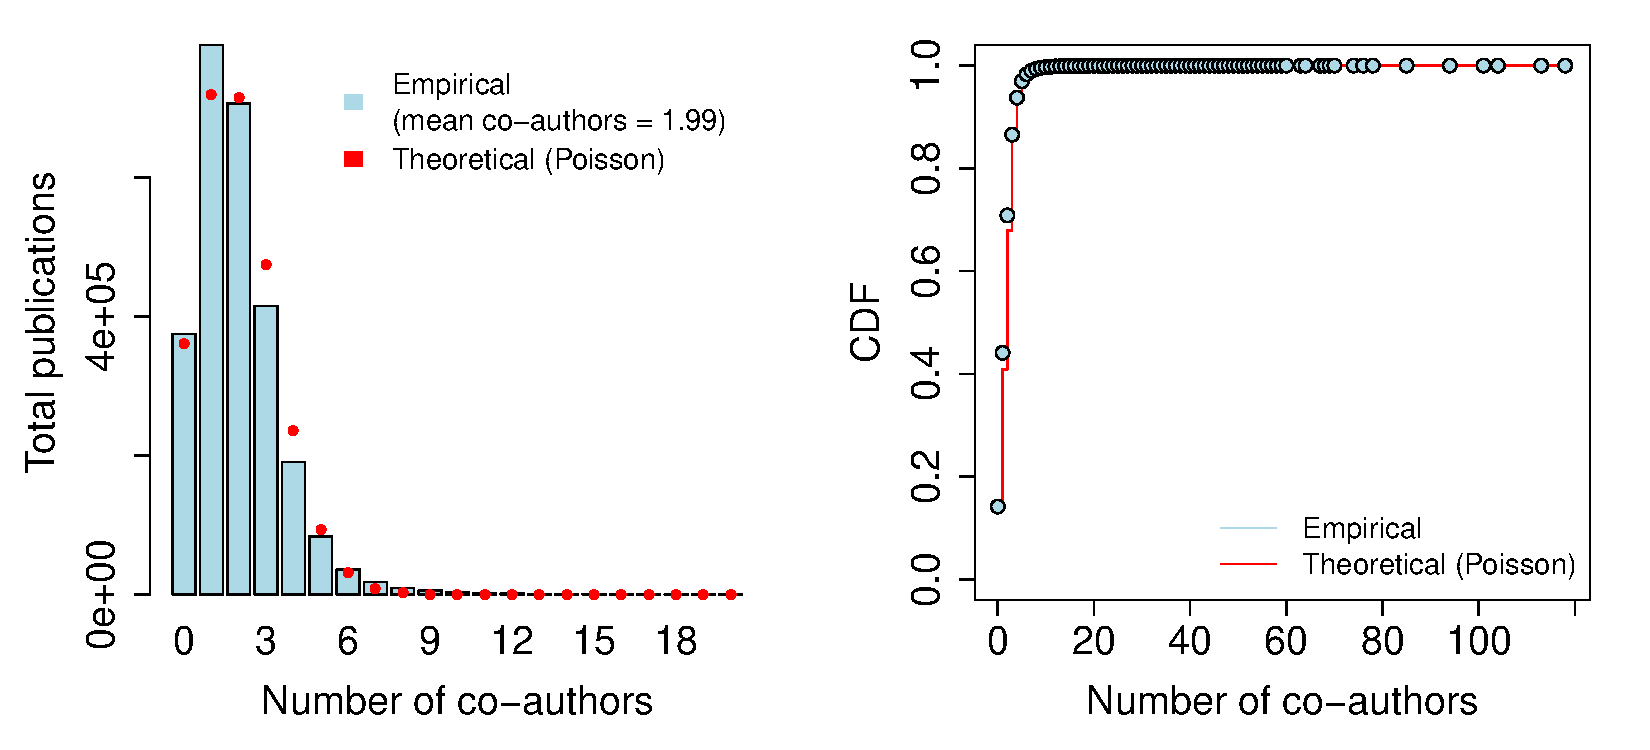
\includegraphics[width=\linewidth]{figures/poisfit}
  \caption{DBLP: Poisson distribution}\label{fig:poisfit}
\end{figure}

The second objective of the experiment was to find authors who are most often in the role of the main author of a publication. The results of this part of the experiment are to be understood only as an estimate based on the above-mentioned assumptions about the main author. Empirical distribution, together with the theoretical value of the Poisson distribution for the first fifteen authors with the highest number of publications in the role of the first author, is shown in Figure \ref{fig:top15}.

\begin{figure}[ht]
\centering
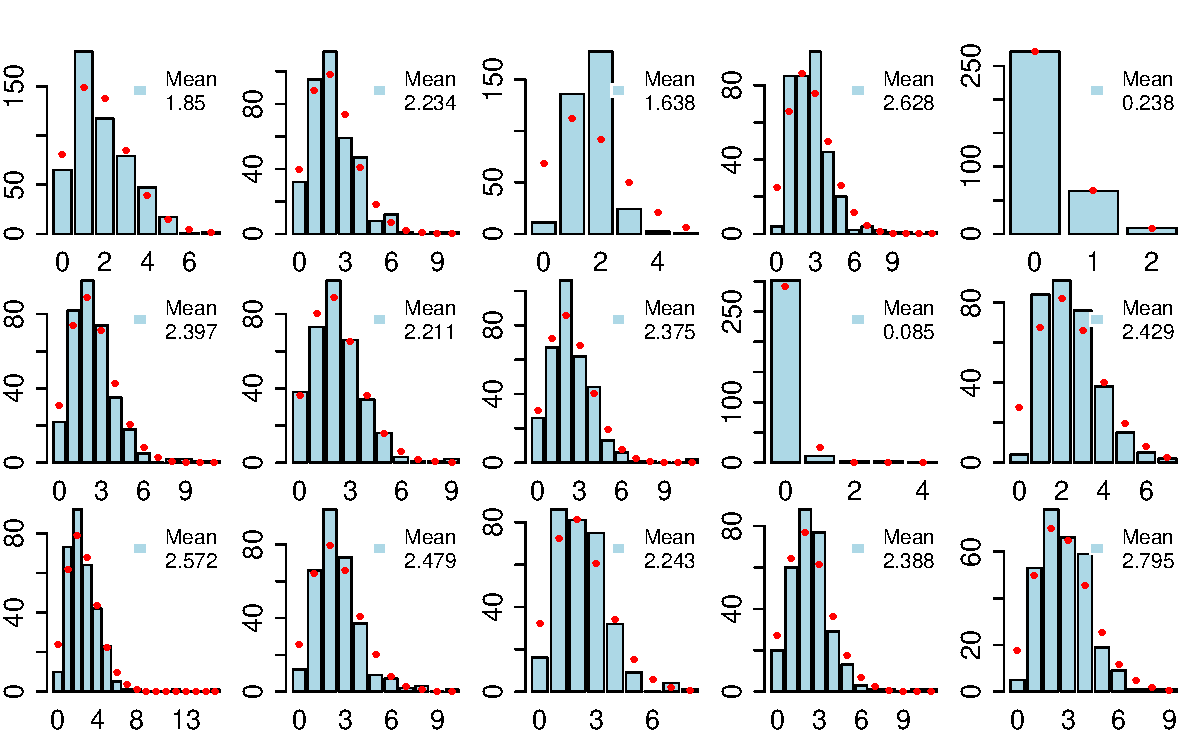
\includegraphics[width=\linewidth]{figures/proactive_coauthors_top15}
  \caption{Co-authors histograms for top 15 authors (by number of publications)}
	\label{fig:top15}
\end{figure}

\subsection{Hypothesis}
Results of the analysis of the DBLP dataset can not be easily generalized. However, experiments have shown quite clearly that the probability of a publication with a certain number of co-authors follows the Poisson distribution. If we extend thoughts about the main author by what kind and how many different co-authors he/she has, we may divide co-authors into three groups. In the first group are authors with whom the main author has previously published. In the second group are those who have previously published but not yet together with the main author. In the third group are new authors, i.e. those who have no previous publications. We can then formulate a hypothesis, based on which we define the new network model in the next part of the paper.

\bigbreak
\textbf{Hypothesis}
\begin{enumerate}
	\item The variables describing the number of co-authors in different groups are independent random variables.
  \item Just as the total number of co-authors, these variables follow Poisson distribution.
\end{enumerate}

In this paper, we are working with a co-authorship network, which is essentially a collaborative network. Therefore, the presented model can not be taken as a universal model. The model is primarily about a simple simulation of the development of collaborative networks inspired by analyzing the co-authorship network.


\section{Matrix Factorization Model}
\label{sec:model} This section will  present the matrix
factorization model which is used for outlier detection. Before
discussing the model in detail, we present the notations and
definitions.  We represent the corpus of text documents as a bag of
words matrix.  A lowercase or uppercase letter such as $x$ or $X$,
is used to denote a scalar. A boldface lowercase letter, such as
$\mathbf{x}$, is used to denote a vector, and  a boldface uppercase
letter, such as $\mathbf{X}$, is used to denote a matrix. This is
consistent with what is commonly used in much of the data mining
literature. Indices typically start from $1$, unless otherwise
mentioned.  For a $\mathbf{X}$, $\mathbf{x}_{i}$ denotes its
$i^{th}$ column, $\mathbf{y}_j^\intercal$ denotes its $j^{th}$ row
and $x_{ij}$ or $X(i,j)$ or $(X)_{ij}$ denote its $(i,j)^{th}$
element.

For greater expressibility, we have also borrowed certain notations
from matrix manipulation scripts such as Matlab and Octave.  For
example, the notation $max(\mathbf{x})$ returns the maximal element
$x \in \mathbf{x}$ and $max(\mathbf{X})$ returns a vector of maximal
elements from each column $\mathbf{x} \in \mathbf{X}$. Similarly,
$\mathbf{X}(i,:)$ denotes the $i$-th row of the matrix and
$\mathbf{X}(:,i)$ for $i$-th column.  For the  reader's convenience,
the notations  used in the paper are summarized in  Table
\ref{table:notations}.

Let $\mathbf{A}$ be the matrix representing the underlying data. In
the context of a text collection, this corresponds to a
term-document matrix, where terms correspond to rows and documents
correspond to columns. In other words, $a_{ij}$ denotes the number
of times the term $i$ appears in document $j$.  Generally, we
can write $\mathbf{A}$ as follows:
\begin{equation}
\mathbf{A} = \mathbf{L_0} + \mathbf{Z_0}.
\end{equation}

\begin{figure}
\scalebox{0.34}[0.29]{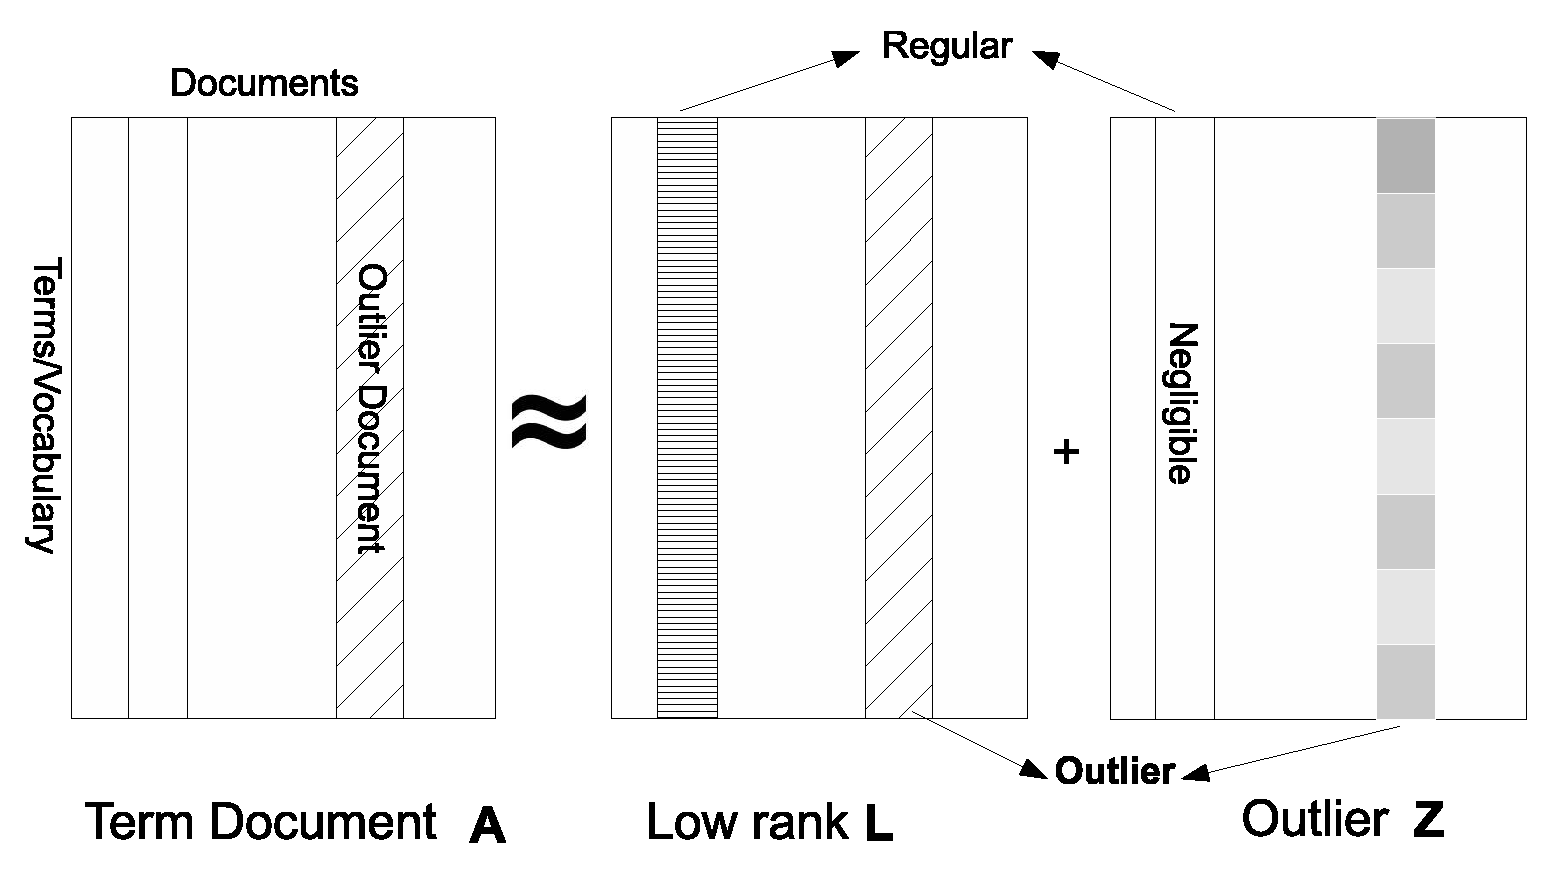
\includegraphics{outlieroverview.eps}}
\caption{Text Outliers Using NMF} \label{fig:outlieroverview}
\end{figure}

Here, $\mathbf{L_0}$ is  a low rank matrix and $\mathbf{Z_0}$
represents the matrix of  outlier entries. Typically, the matrix
$\mathbf{L_0}$ represents the documents created by a lower rank
generative process (such as that modeled by pLSI), and the parts of
the documents that do not correspond to the generative process are
represented as part of the matrix $\mathbf{Z_0}$.   In real world
scenarios, the outlier matrix $\mathbf{Z_0}$  contains  entries
which are very close to zero, and  only a small number of entries
have {\em significantly} non-zero values. These significantly
nonzero entries are often present in only a small fraction of the
columns. Columns which are fully representable in terms of factors
are consistent with the low rank behavior of the data, and therefore
{\em not} outliers. The rank of $\mathbf{L}_0$ is not known in
advance, and it can be expressed in terms of its underlying factors.
$$
\mathbf{L}_0 \approx \mathbf{W}_0\mathbf{H}_0
$$
Here, the two matrices   have dimensions $\mathbf{W}_0 \in
\mathbb{R}^{m \times r}_+$, $\mathbf{H}_0 \in \mathbb{R}^{r \times
n}_+$, and $r \le rank(\mathbf{L}_0)$. The matrices $\mathbf{W}_0$
and  $\mathbf{H}_0$ are non-negative, and this provides
interpretability in terms of being able to express a document as a
non-negative linear combination of the relevant basis vectors, each
of which in itself can be considered a frequency-annotated bag of
words (topics) because of its non-negativity.  Specifically,
$\mathbf{H_0}$ corresponds to the coefficients for the basis matrix
$\mathbf{W_0}$. Intuitively, this corresponds to the case that every
document
 $\mathbf{a}_i$, is represented as the linear combination of
the $r$ topics. In cases, where this is {\em not} true, the document
is an outlier, and those  unrepresentable sections of the matrix are
captured by the non-zero entries in the   $\mathbf{Z_0}$ matrix. In
real scenarios,  the entries in  this matrix are often  extremely
skewed, and the small number of non-zero entries very obviously
expose the outliers.  The decomposition of the matrix into different
component is pictorially illustrated  in Figure
\ref{fig:outlieroverview}.

In order to determine the best low rank factorization, one must try
to optimize the  aggregate  values of the residuals in  the matrix.
This can of course be done in a variety of ways, depending upon the
goals of the underlying factorization process.  We model the
determination of the matrices $\mathbf{W}$,$\mathbf{H}$, and
$\mathbf{Z}$, as the following optimization problem:
\begin{equation}\label{l12norm}
(\mathbf{W}_0,\mathbf{H}_0;\mathbf{Z}_0)=\argmin_{\mathbf{W}\ge0,\mathbf{H}\ge0; \mathbf{Z}}  \frac{1}{2}\norm{\mathbf{A}-\mathbf{W}\mathbf{H}-\mathbf{Z}}_F^2 + \alpha\norm{\mathbf{Z}}_{1,2}
\end{equation}

The specific location of outliers in each column does not have a
closed form solution, since the $\ell_{1,2}$-norm penalty is applied
to $\mathbf{Z}$.   The   logic for applying the $\ell_{1,2}$-norm in
the context of the outlier detection problem is as follows.  Each
entry in the $\mathbf{Z}$ corresponds to a term in a document,
whereas we are interested in the outlier behavior of entire
document. This aggregate outlier behavior of the document $x$ can
be modeled with the $\ell_2$ norm score of a particular column
$\mathbf{z}_x$. In a real scenario,  if a large segment  of a
document $x$ is not representable as the linear combination of the
$r$ topics through $\mathbf{L_0}$, the corresponding column
$\mathbf{z}_x$ in the matrix $\mathbf{Z}$ will be compensated by
having more entries in its column.  In other words, we will  have a
higher $\ell_2$ value for the corresponding column $\mathbf{z}_x$,
and this corresponds to a higher outlier score.
 Furthermore, the  $\ell_{1,2}$-norm penalty on $\mathbf{Z}$
defines the sum of the $\ell_2$ norm outlier scores over all the
documents.  Therefore,  the optimization problem essentially tries
to find the best model,  an important component of which is to
minimize the sum of the outlier scores over all documents.  While a
variety of different  (and more commonly used) penalties such as the
Frobenius norm are available for matrix factorization models, we
have chosen the $\ell_{1,2}$-norm penalty because of its intuitive
significance in the context of the outlier detection problem, and
its tendency to create skewed outlier scores across the columns of
the matrix. As we will see in the next section, this comes at the
expense of a formulation which is more difficult to solve
algorithmically.

For high dimensional data, sparse coefficients are desirable for
obtaining an interpretable low rank matrix $\mathbf{W}\mathbf{H}$.
For this purpose, we add the $\ell_1$-penalty on $\mathbf{H}$:
\begin{equation}\label{outlier}
\min_{\mathbf{W}\ge0,\mathbf{H}\ge0; \mathbf{Z}}  \frac{1}{2}\norm{\mathbf{A}-\mathbf{W}\mathbf{H}-\mathbf{Z}}_F^2 + \alpha\norm{\mathbf{Z}}_{1,2} + \beta\norm{\mathbf{H}}_{1}
\end{equation}
 The constant $\alpha$ defines the weight
for the outlier matrix $\mathbf{Z}$ over the recovery of the low
rank space $\mathbf{L}$ and the sparsity term. In the case of
outlier detection in text documents, we give more weight for the
outlier matrix over the low rank representation $\mathbf{L}$. This
problem does not have a closed form solution, and
 therefore we cannot  directly recover the low rank
matrix $\mathbf{W}\mathbf{H}$ in closed form. However, we can
recover the column space. Without non-negativity constraints, this
property is also known as the rotational invariant property
\cite{ding06,xu12}. This particular formulation of the matrix
factorization model is a bit different from the commonly used
formulations, and off-the-shelf solutions do not directly exist for
this scenario. Therefore, in a later section, we will carefully
design an algorithm with the use of block coordinate descent for
this problem.

In order to understand the modeling of the outliers better, we
present the readers with a toy example from a real world data set,
to show how  skewed the typical values of the corresponding column
$\mathbf{z}(x)$ may be in real scenarios.  In this case, we used the
{\em BBC} dataset\footnote{\url{http://mlg.ucd.ie/datasets/bbc.html}}.
\ramki{This dataset consists of documents from BBC news website corresponding
to stories in area business, entertainment, politics, sport, tech from 2004-2005 . 
%We ran our algorithm \algo explained in the next Section
%\ref{sec:algorithm} to find the matrices $\mathbf{W,H}$ and $\mathbf{Z}$.
We took all the documents from business and politics  and 50
documents from tech labeled as outliers. We randomly permuted the columns to 
shuffle the outliers in the matrix to avoid any spatial bias}. 
We computed the $\mathbf{Z}$ matrix
and   generated the $\ell_2$ scores of the columns of outlier matrix
$\mathbf{Z}$. Figure \ref{fig:outlierz} shows the outlier($\ell_2$)
scores of the documents. The $X$-axis illustrates the index of the
document, and the $Y$-axis illustrates the outlier score. It is
evident that  the scores for some  columns are so close to zero,
that they cannot even be seen on the diagram drawn to scale. These
columns also happened to be the non-outlier/regular documents of the collection.
Such documents $\mathbf{a}_x \in \mathbb{R}^m$ correspond to the low
rank space, and  are approximately representable as  a product of
the basis  matrix $\mathbf{W}$ with the corresponding column vector
of coefficients $\mathbf{h}_x \in \mathbb{R}^r$ drawn from
$\mathbf{H}$. However, the documents that are not representable in
such a low rank space have a large outlier score. From the
distribution of the outlier score, we can also observe that the
scores of outlier documents against non-outliers are clearly
separable, by using a simple statistical mean and standard deviation
analysis. Therefore, while we use the scores to rank the documents
in terms of their outlier behavior, the skew in the entries ensures
that it is often easy to choose a cut-off in order to distinguish
the outliers from the non-outliers.

\begin{figure}
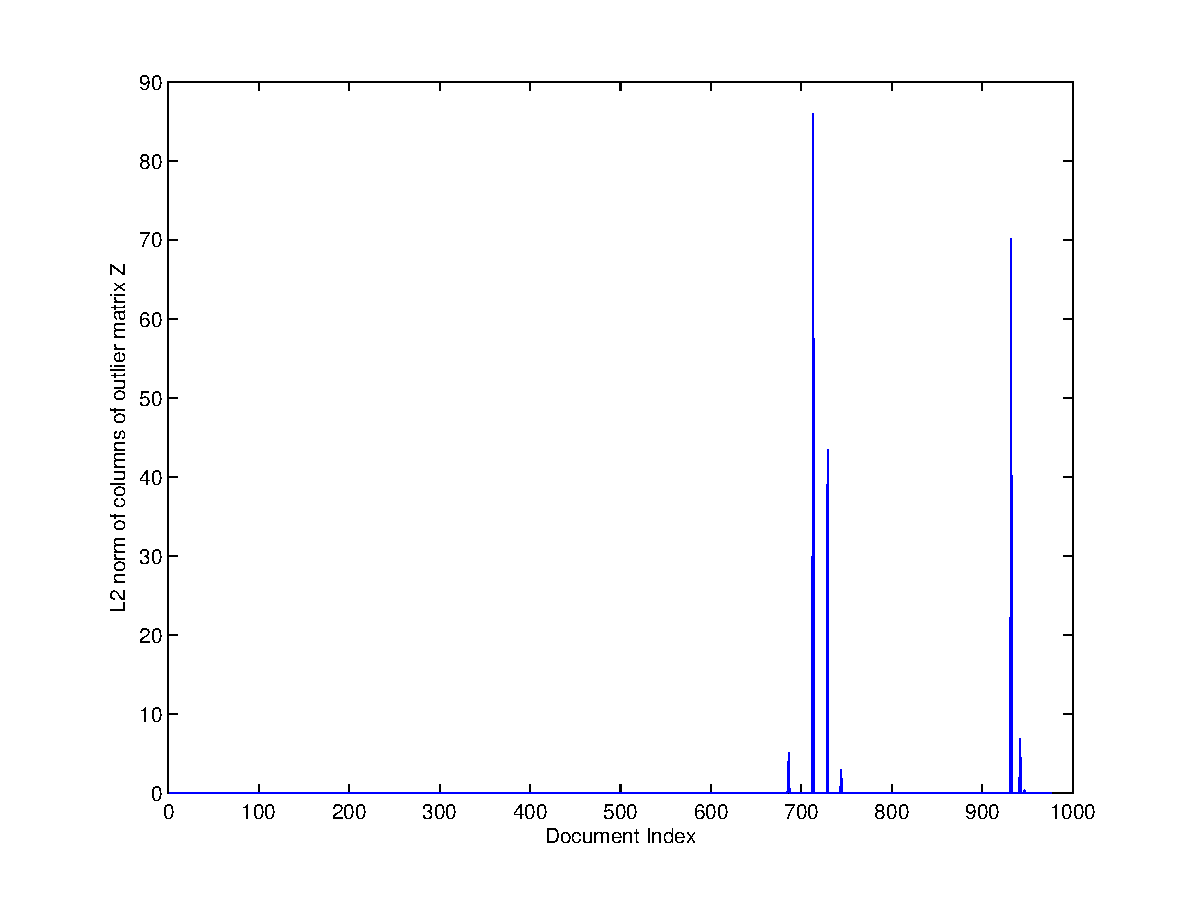
\includegraphics[scale=0.4]{outlierzbbc.eps}
\caption{$\ell_2$ norm of columns of $\mathbf{Z}$ outlier matrix}
\label{fig:outlierz}
\end{figure}



In the following sections, we will analyze the property and
performance of this model \eqref{outlier} for outlier detection
problems.


\section{Experimental Evaluation}
\label{sec:exp}
We are using using three different settings, $Setting = [\lambda_1, \lambda_2, \lambda_3]$, in the experiments. In $Setting_1 = [1.6, 0.35, 0.05]$, the average interaction involved three nodes (a triad), which corresponds approximately to the analyzed co-authorship network. This setting presumes the interaction is dominated by neighbors of the proactive node with the occasional participation of new nodes and rather exceptional participation of existing nodes yet not connected to the proactive node. In $Setting_2 = [3, 6, 1]$ predominate new nodes, and the average number of nodes in interaction is $11$. In $Setting_3 = [0.45, 0.45, 0.1]$ interaction involved two nodes (a dyad) on average, wherein the number of neighbors and new nodes are balanced and new connection occurrences are less likely.

\begin{figure}[ht]
	\centering
  \begin{subfigure}{2.7cm}
    \centering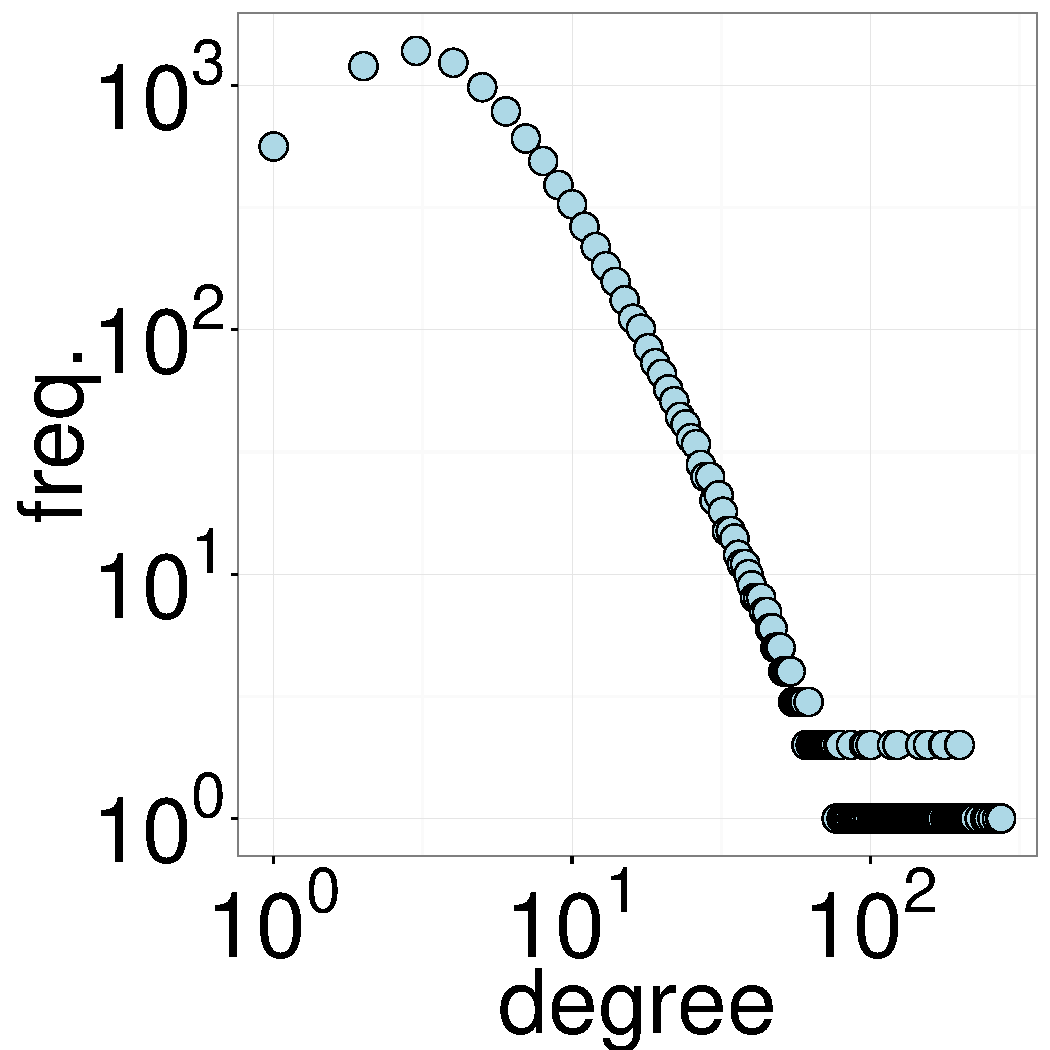
\includegraphics[width=2.5cm]{figures/distr_stupnu_Setting1}
    \caption{$Setting_1$}
  \end{subfigure}
  \begin{subfigure}{2.7cm}
    \centering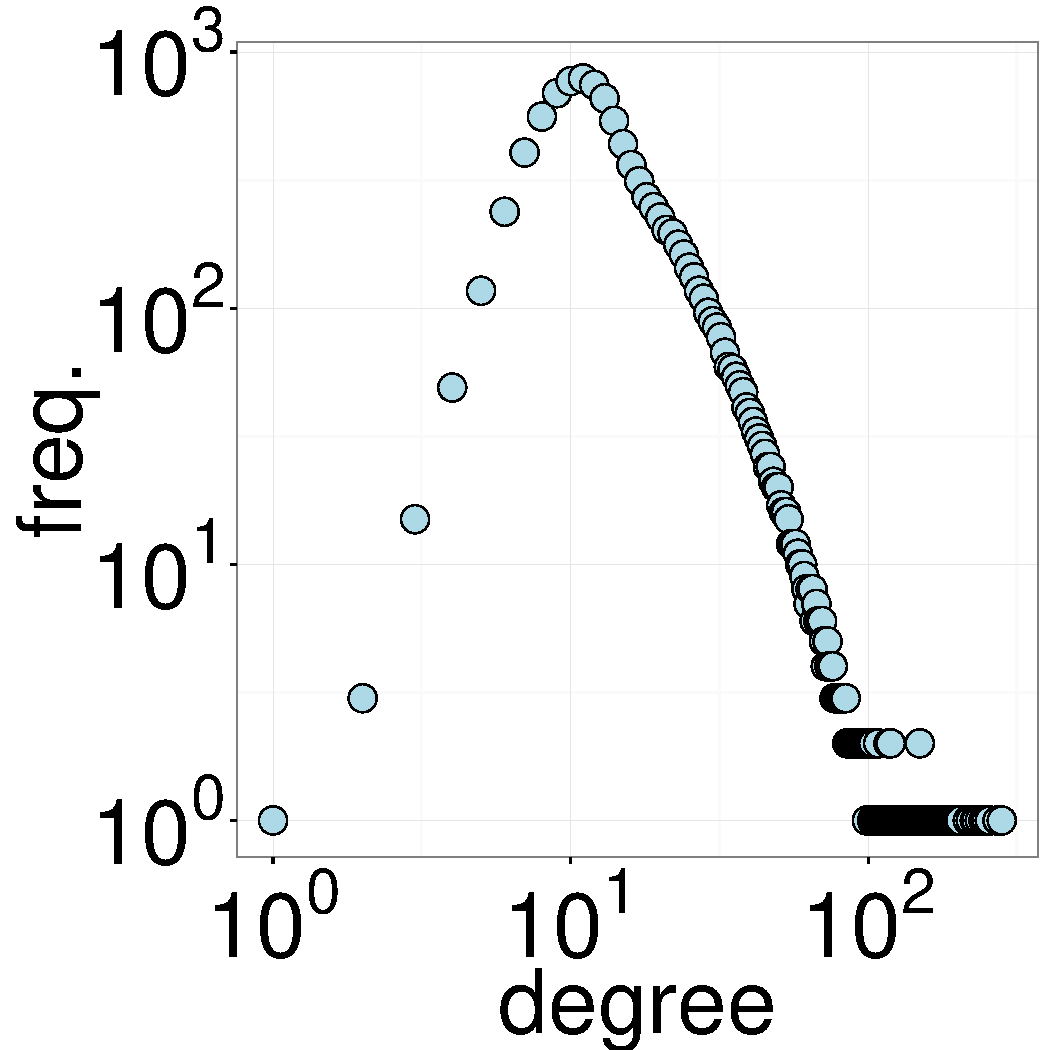
\includegraphics[width=2.5cm]{figures/distr_stupnu_Setting2}
    \caption{$Setting_2$}
		  \end{subfigure}
   \begin{subfigure}{2.7cm}
    \centering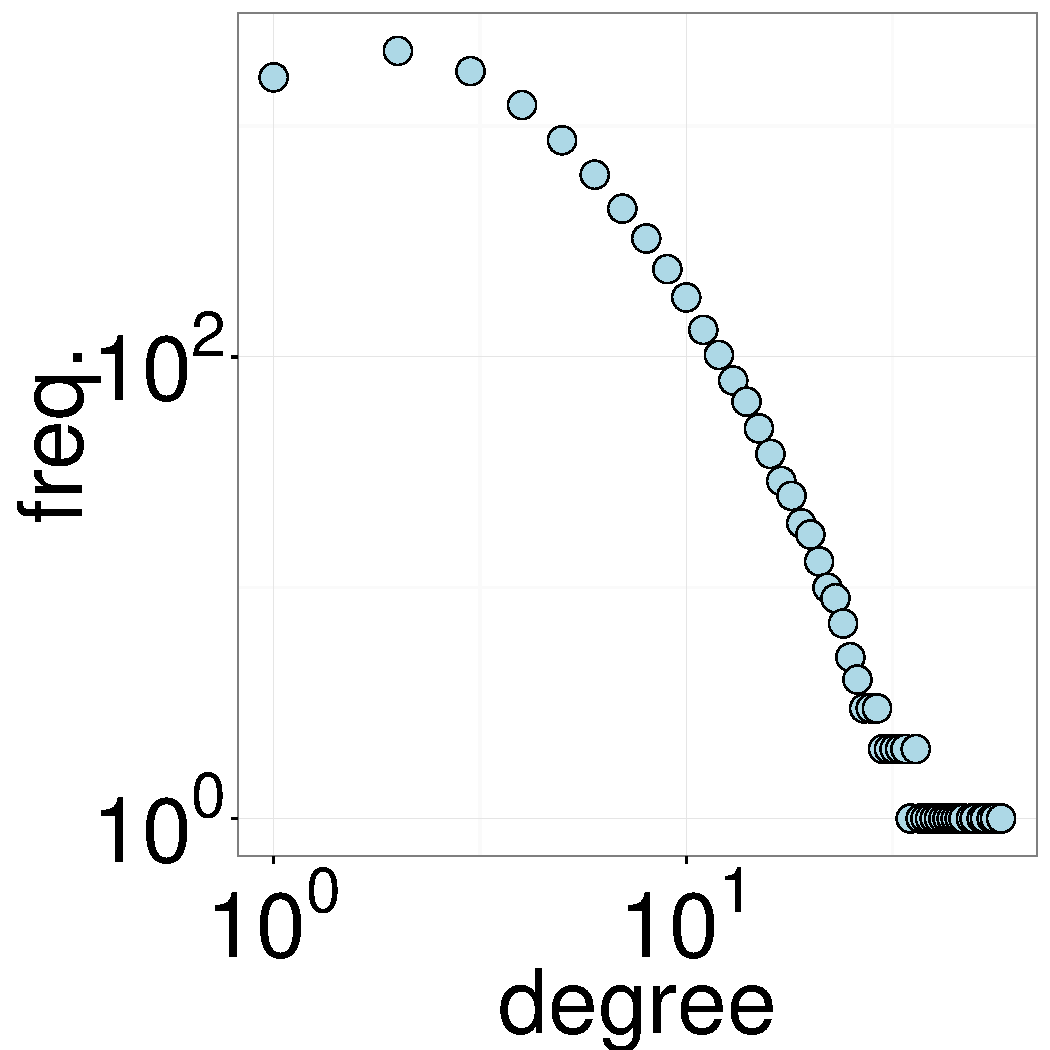
\includegraphics[width=2.5cm]{figures/distr_stupnu_Setting3}
    \caption{$Setting_3$}
  \end{subfigure}
	\caption{Degree distribution}
\label{fig:DD}
\end{figure}

\begin{figure}[ht]
	\centering
  \begin{subfigure}{2.7cm}
    \centering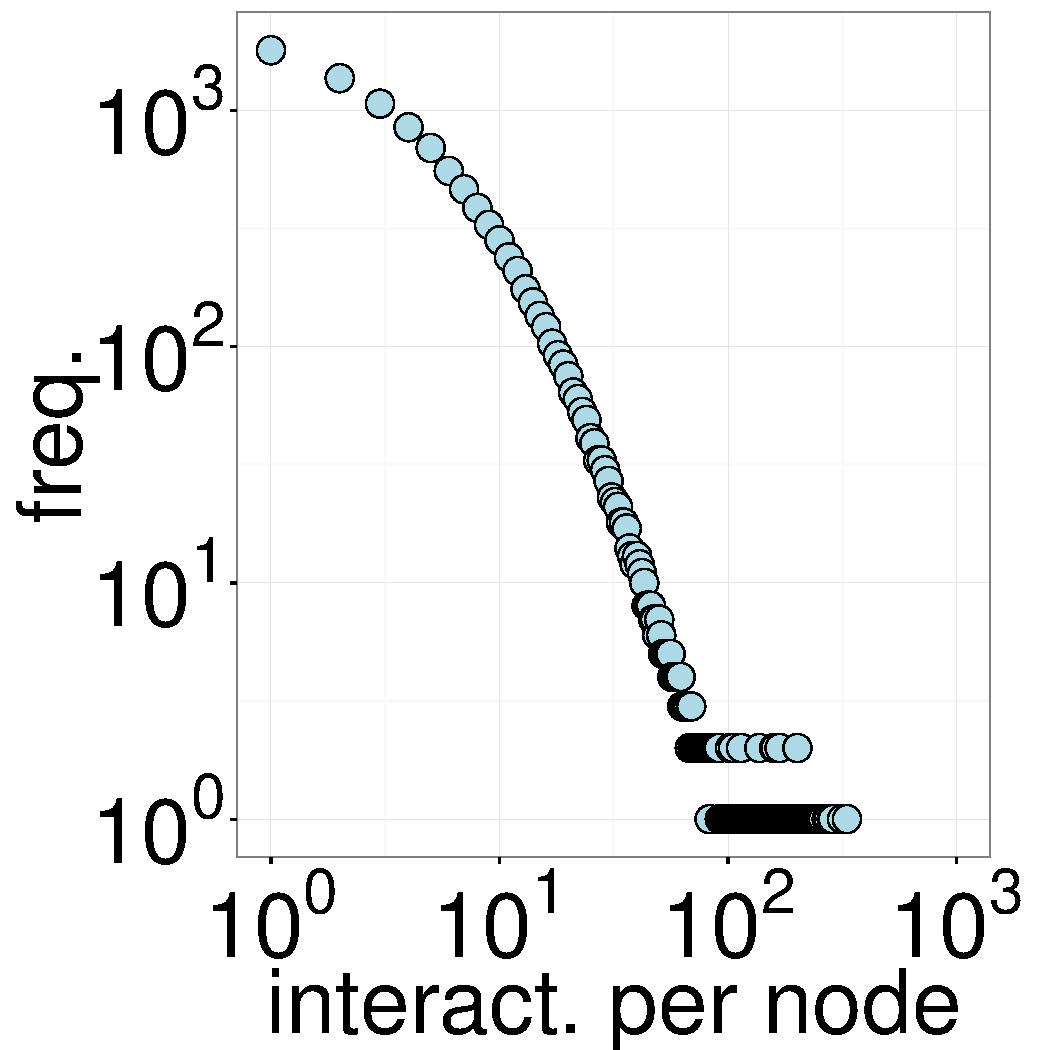
\includegraphics[width=2.5cm]{figures/inter_per_vert_Setting1}
    \caption{$Setting_1$}
  \end{subfigure}
  \begin{subfigure}{2.7cm}
    \centering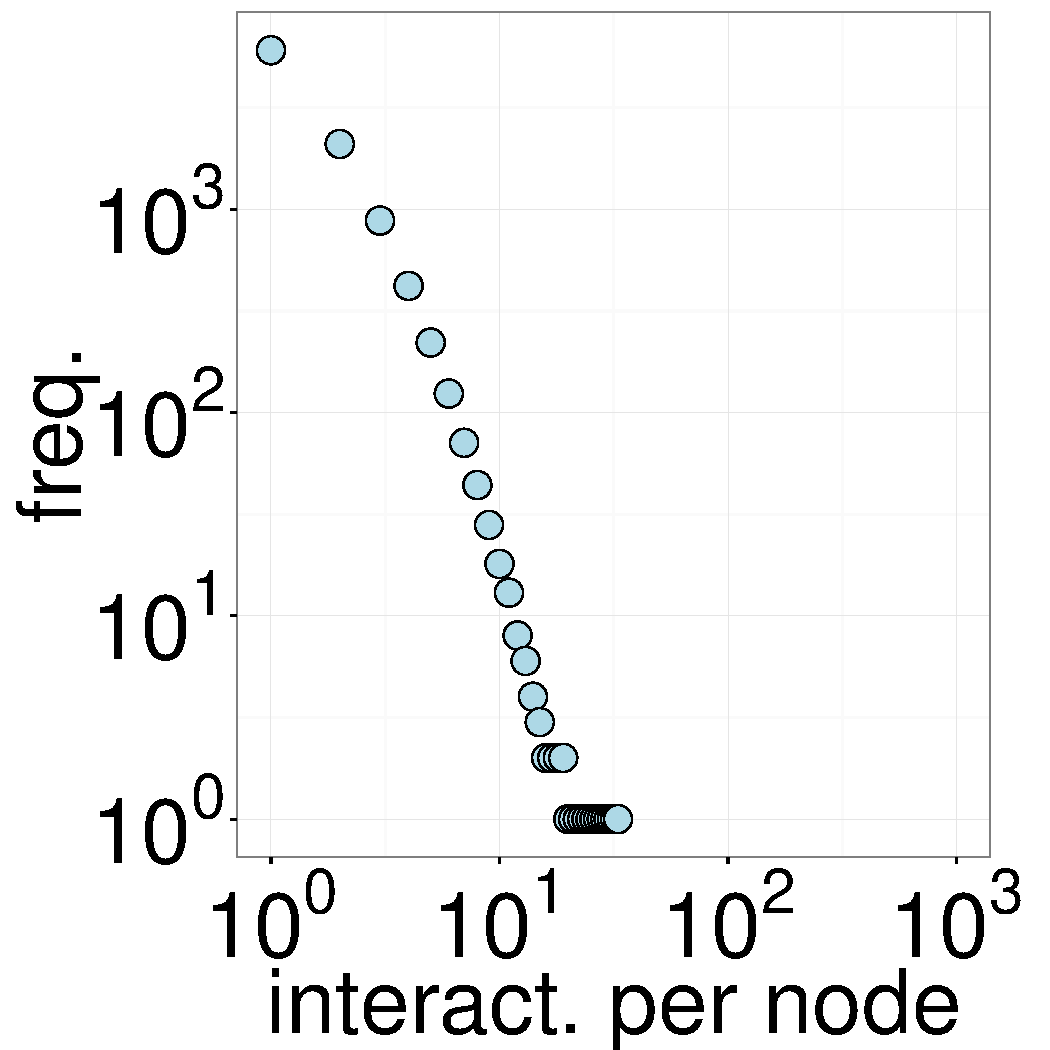
\includegraphics[width=2.5cm]{figures/inter_per_vert_Setting2}
    \caption{$Setting_2$}
		  \end{subfigure}
   \begin{subfigure}{2.7cm}
    \centering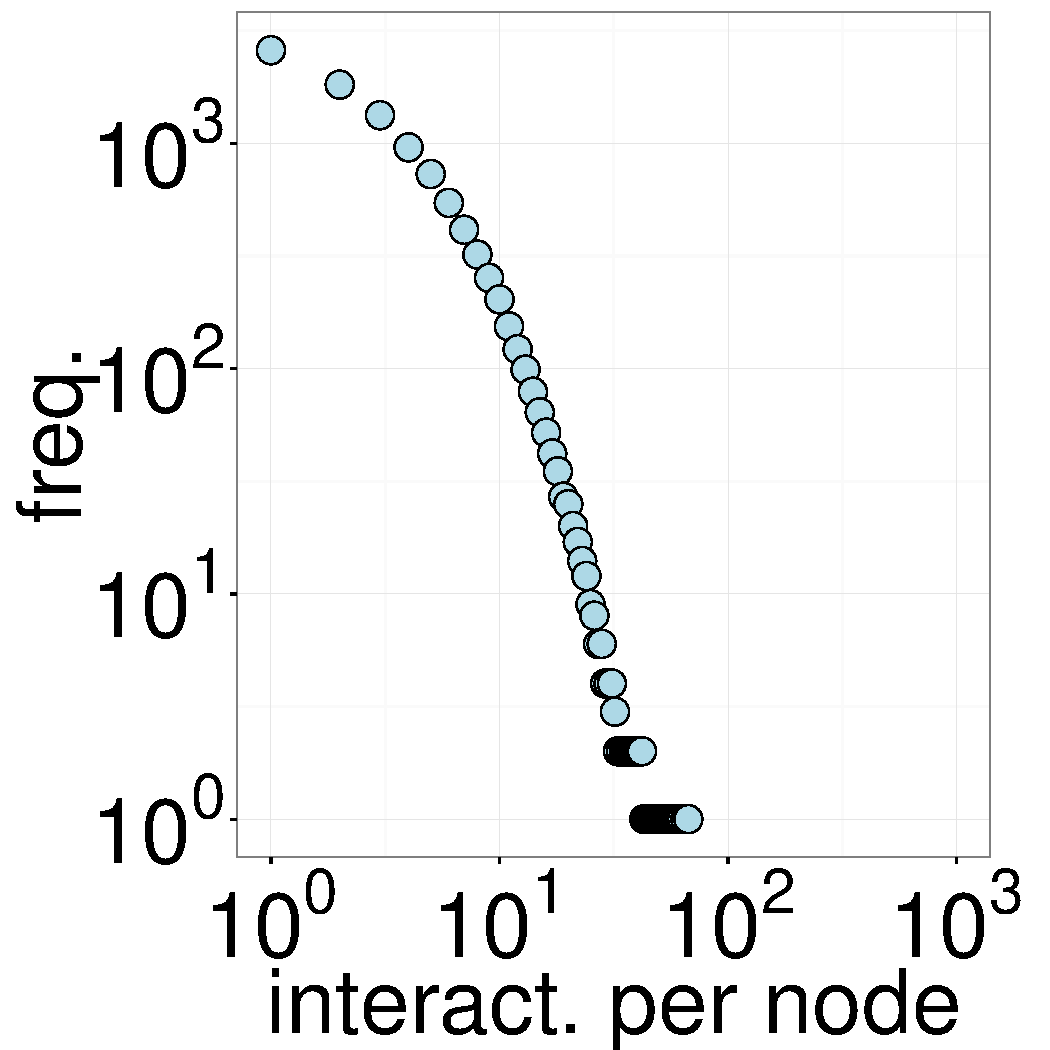
\includegraphics[width=2.5cm]{figures/inter_per_vert_Setting3}
    \caption{$Setting_3$}
  \end{subfigure}
	\caption{Interactions per	node}
\label{fig:IpN}
\end{figure}

\begin{figure}[ht]
	\centering
  \begin{subfigure}{2.7cm}
    \centering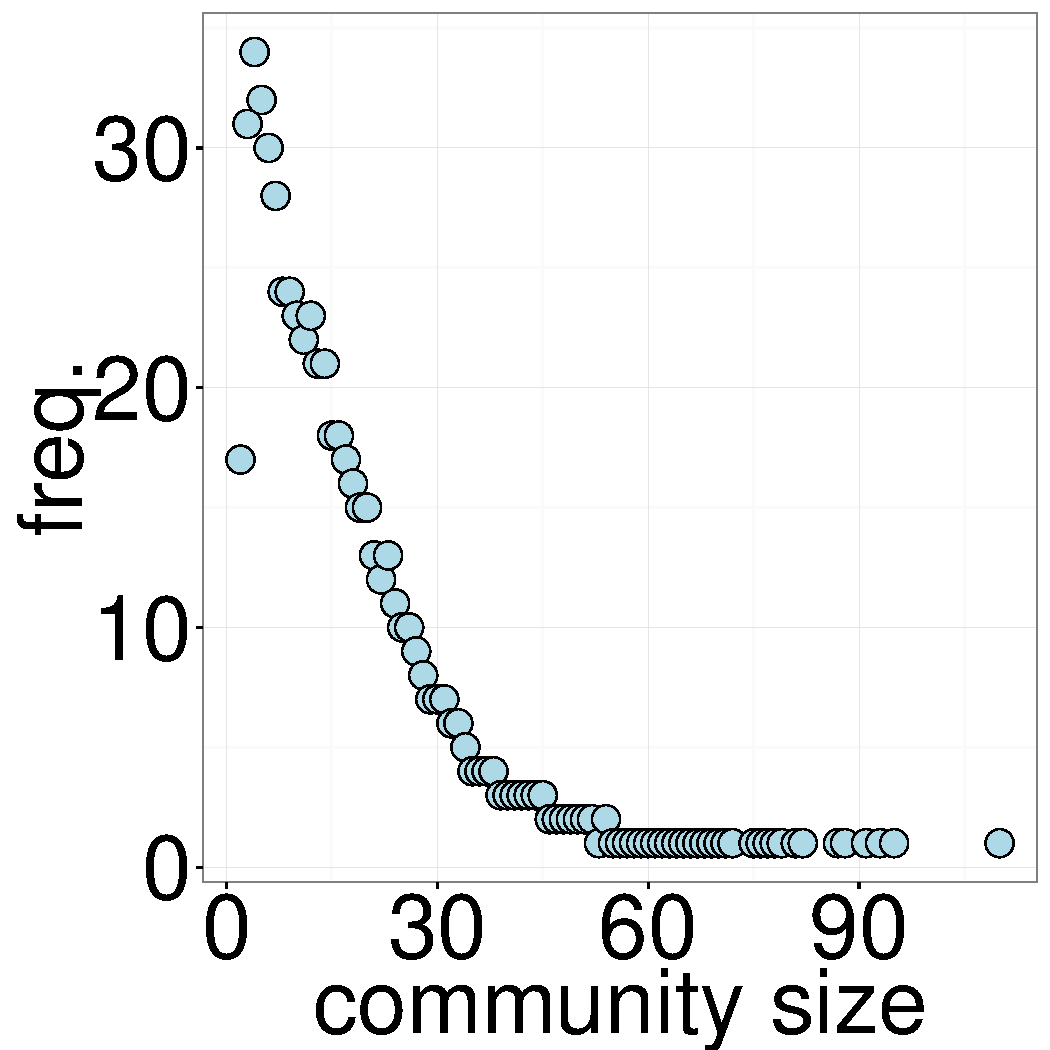
\includegraphics[width=2.5cm]{figures/dist_vel_komf_Setting1}
    \caption{$Setting_1$}
  \end{subfigure}
  \begin{subfigure}{2.7cm}
    \centering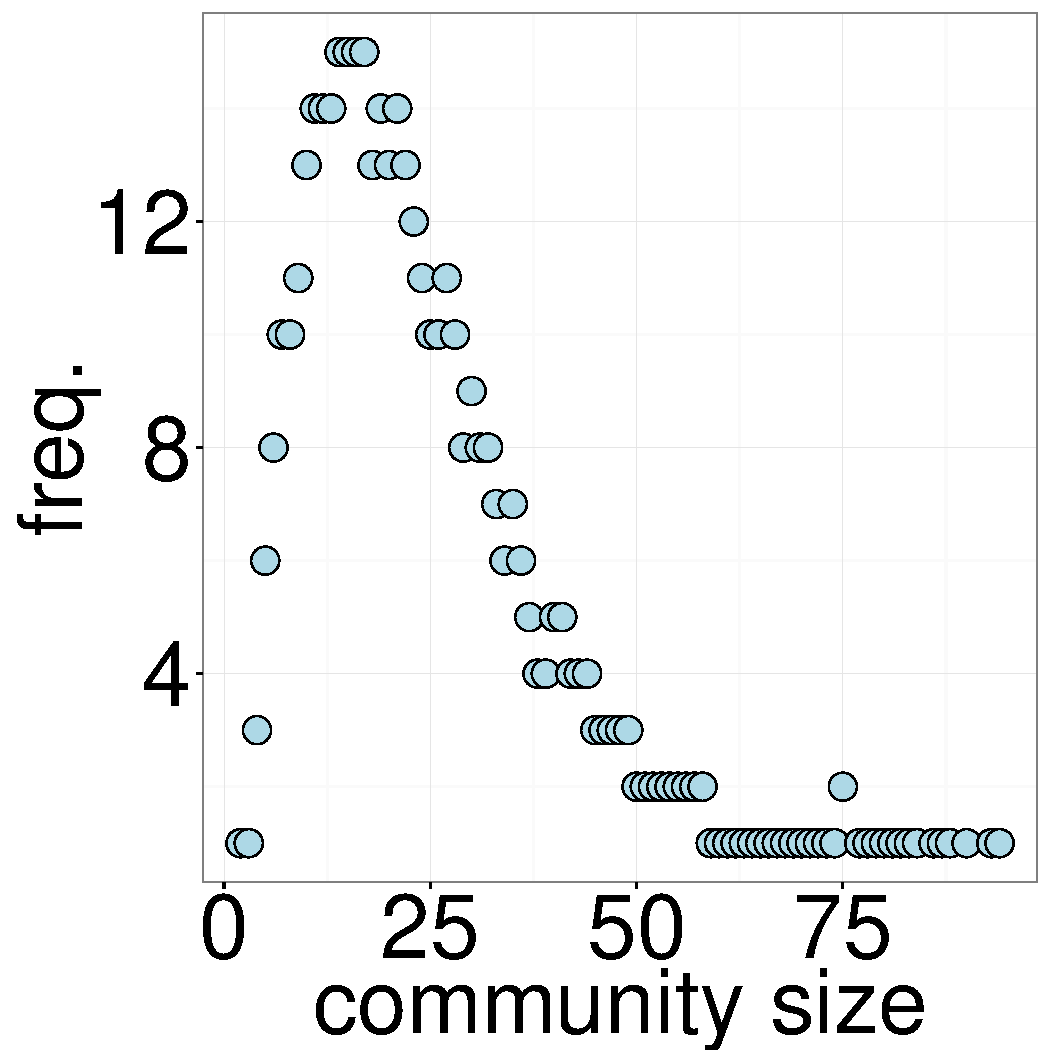
\includegraphics[width=2.5cm]{figures/dist_vel_komf_Setting2}
    \caption{$Setting_2$}
		  \end{subfigure}
   \begin{subfigure}{2.7cm}
    \centering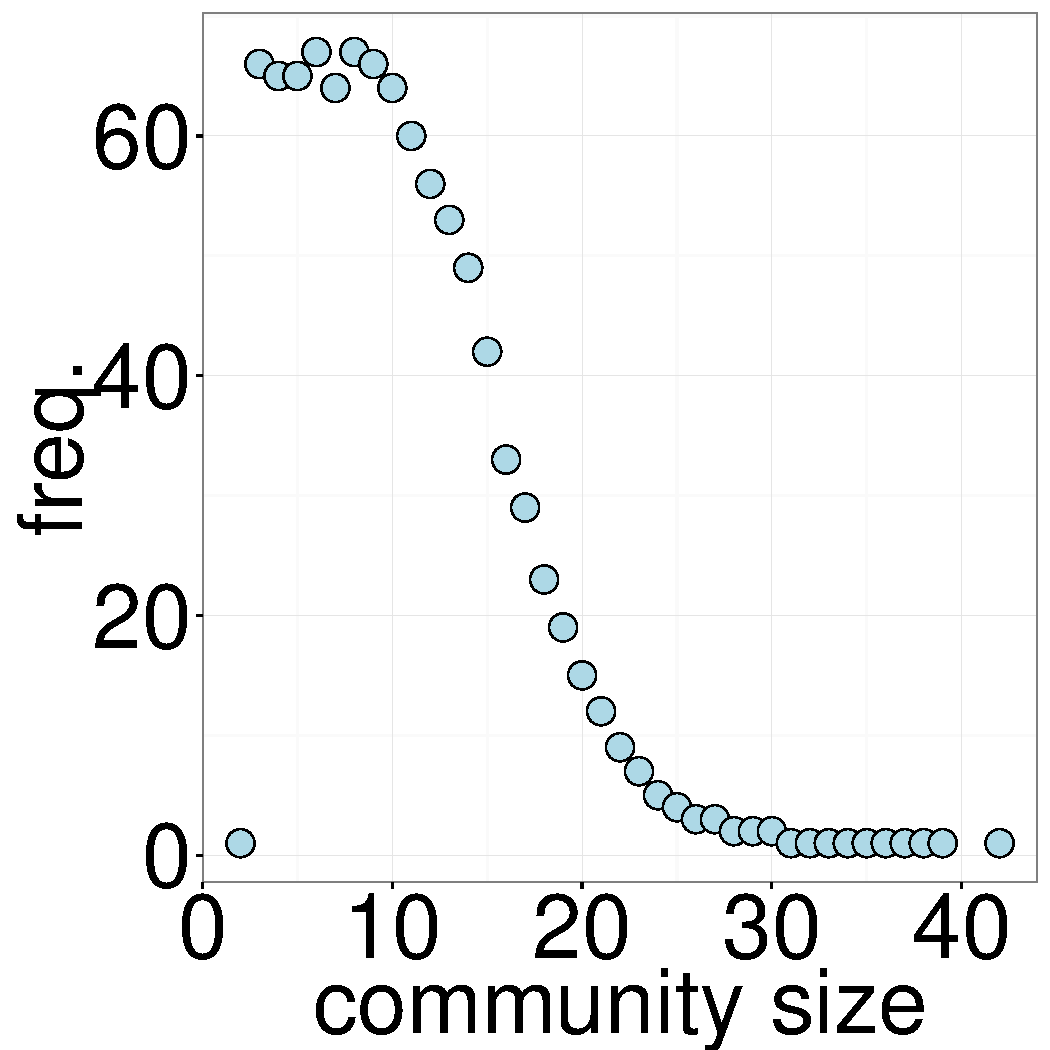
\includegraphics[width=2.5cm]{figures/dist_vel_komf_Setting3}
    \caption{$Setting_3$}
  \end{subfigure}
	\caption{Community size}
\label{fig:ComSize}
\end{figure}


\subsection{Properties of Generated Network}

\begin{table*}[ht]
  \centering
  \caption{Global properties}
		\begin{tabular}{|c|r|rrrrrrrrrrr|}
\hline
Setting &  & $n$ & $m$ & $<$k$>$ &  $<$l$>$ & $l_{max}$ & $CC$ & $r$ & $com_{IM}$ & $com_L$ & $Q_{IM}$ & $Q_L$ \\ 
\hline
$Setting_1$ & mean & 10001.10 & 40108.97 & 8.0209 & 4.8101 & 12.07 & 0.6555 & 0.14522 & 609.40 & 54.70 & 0.6424 & 0.7119 \\ 
& sd & 0.31 & 398.80 & 0.0797 & 0.0421 & 0.64 & 0.0029 & 0.01769 & 12.37 & 7.04 & 0.0062 & 0.0085 \\ 
\hline	
$Setting_2$ & mean & 10003.87 & 88620.40 & 17.7172 & 4.2369 & 8.43  & 0.8087 & 0.12961 & 422.60 & 42.90 & 0.6772 & 0.7334 \\ 
& sd & 1.53 & 797.95 & 0.1600 & 0.0277 & 0.63  & 0.0018 & 0.00913 & 10.30 & 2.78 & 0.0049 & 0.0067 \\ 
\hline
$Setting_3$ & mean & 10001.17 & 21494.57 & 4.2984 & 6.8965 & 16.23 & 0.4784 & 0.19907 & 953.30 & 68.70 & 0.7276 & 0.8129 \\ 
&  sd & 0.46 & 142.64 & 0.0285 & 0.0609 & 0.63 & 0.0044 & 0.01222 & 15.55 & 3.19 & 0.0035 & 0.0038 \\ 
\hline
\end{tabular}%
  \label{tab:gp}%
\end{table*}%
\begin{table}[ht]
  \centering
  \caption{Interactions}
\begin{tabular}{|r|r|rrr|}
	\hline
Setting & & $I$ & $<$i$>$ & $<$s$>$ \\ 
\hline
$Setting_1$ & mean & 28561.90 & 8.0887 & 2.8323 \\ 
&  sd & 278.93 & 0.0817 & 0.0082 \\ 
\hline	
$Setting_2$ & mean & 1664.53 & 1.8278 & 10.9860 \\ 
& sd & 17.69 & 0.0115 & 0.0824 \\
\hline	
$Setting_3$ & mean & 22204.43 & 4.3772 & 1.9716 \\ 
& sd & 202.06 & 0.0292 & 0.0069 \\ 
\hline
	\end{tabular}%
  \label{tab:interact}%
\end{table}%

In the first experiment, we show the properties of networks generated with different settings. We generated for each setting $100$ networks with approximately $10000$ nodes. Table \ref{tab:gp} summarizes average values (and standard deviation) of measured properties for each setting. Measured properties include number of nodes $n$ and edges $m$, average degree $<$k$>$, average shortest path length $<$l$>$, diameter $L_{max}$, average clustering coefficient $CC$, assortativity $r$, number of communities detected by Infomap \cite{rosvall2009map} $com_{IM}$ and Louvain \cite{blondel2008fast} $com_L$ algorithm, and corresponding modularities $Q_{IM}$ and $Q_L$, respectively. Table \ref{tab:interact} contains average values associated with the temporality of the network, i.e. total number of interactions $I$, average number of interactions $<$i$>$ and average number of nodes in interaction $<$s$>$. Figures \ref{fig:DD}-\ref{fig:ComSize} show degree distribution, number of interactions distribution and distributions of community size detected by Infomap algorithm.

The experiment indicates that all three settings generate networks with small-world and scale-free characteristics. The first and second setting have generated networks of high average clustering coefficient. Networks have a tendency to be assortative. Assortativity values correspond to all settings to the values known from social networks \cite{newman2002assortative}. Generated networks also have community structure and a high modularity for all settings.

\begin{figure}[ht]
\centering
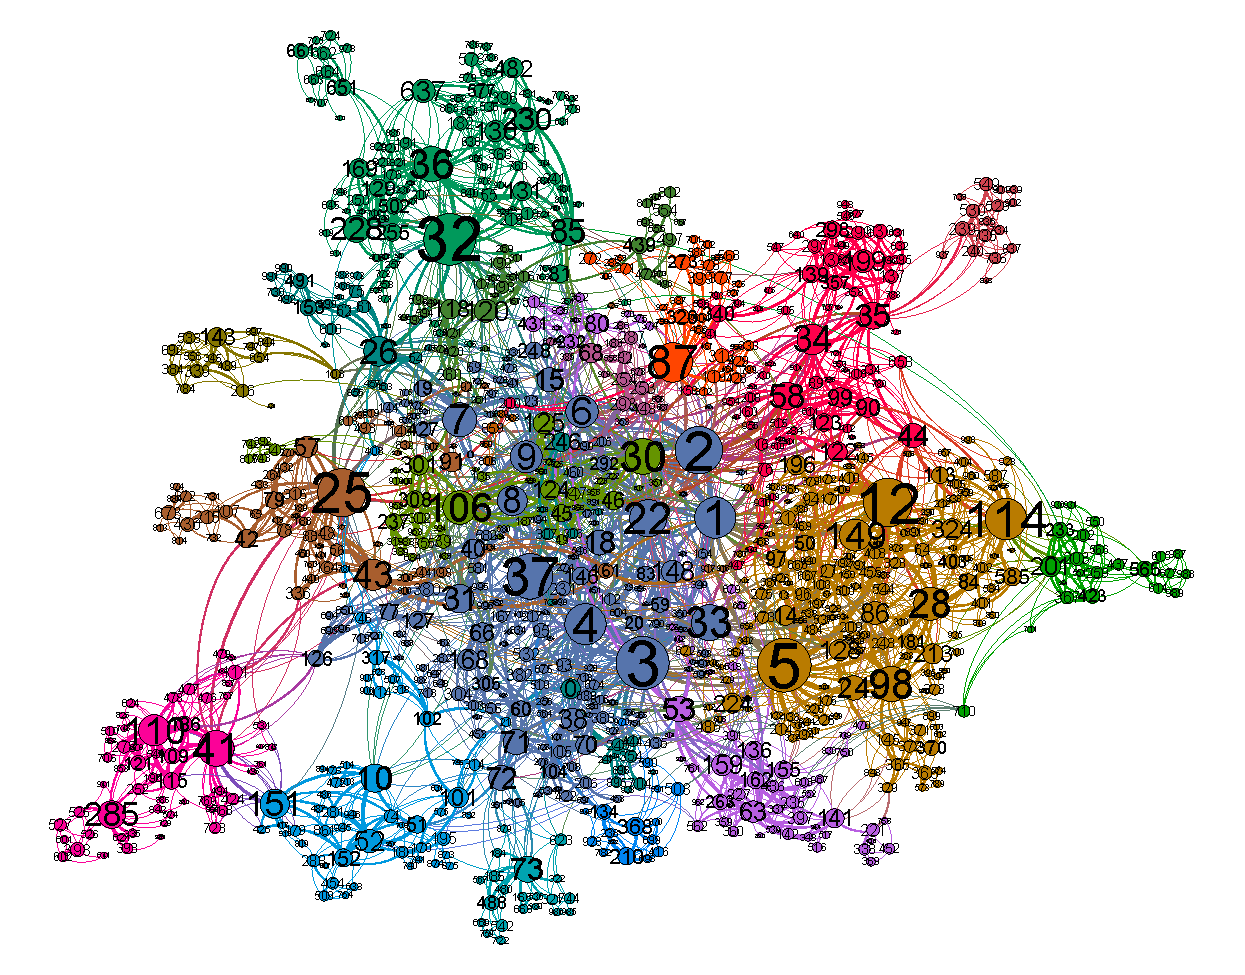
\includegraphics[width=\linewidth]{figures/setting1_1000}
  \caption{Network: 1000 nodes, $Setting_1$}
	\label{fig:Set1000}
\end{figure}

Figure \ref{fig:Set1000} shows a network with $1000$ nodes and $3599$ edges generated with $Setting_1$. A total of $2830$ interactions took place. The size of nodes and strength of edges correspond to the number of interactions they took part in, the labels indicate the order in which nodes were created. The network has an overlapping community and core-periphery structure. Colored 19 communities were detected by Louvain method, modularity is $0.746$.

\subsection{Evolution of Generated Network}
The subject of the second experiment is one network generated with $Setting_1$. The aim is to show the development of network properties during its growth. The values for each characteristic are measured when the network has $10, 20, 50, 100$, ..., and $10000$ nodes. The results are summarized in Table \ref{tab:Evolut}.

\begin{table*}[ht]
  \centering
  \caption{Evolution of network properties}
	\begin{tabular}{|r|rrrrrrrrrr|}

\hline
  $n$ & $m$ & $<$k$>$ &  $<$l$>$ & $l_{max}$ & $CC$ & $r$ & $com_{IM}$ & $com_L$ & $Q_{IM}$ & $Q_L$ \\
\hline
  10 & 27.00 & 5.4000 & 1.4000 & 20 & 0.8195 & -0.41738 & 1 & 3 & 0.0000 & 0.0590 \\ 
 20 & 53.00 & 5.3000 & 2.0684 & 5 & 0.5804 & -0.09355 & 2 & 4 & 0.0361 & 0.2398 \\ 
  50 & 184.00 & 7.3600 & 2.5004 & 7 & 0.6248 & -0.00886 & 5 & 5 & 0.2957 & 0.3742 \\ 
100 & 388.00 & 7.7600 & 2.8731 & 6 & 0.6793 & 0.09177 & 11 & 9 & 0.4259 & 0.4613 \\ 
 200 & 812.00 & 8.1200 & 3.1859 & 7 & 0.6824 & 0.05107 & 20 & 11 & 0.5002 & 0.5121 \\ 
500 & 2112.00 & 8.4480 & 3.6095 & 8 & 0.6394 & 0.11911 & 44 & 11 & 0.5540 & 0.5849 \\ 
 1000 & 4053.00 & 8.1060 & 3.9402 & 9 & 0.6592 & 0.14528 & 83 & 17 & 0.5812 & 0.6341 \\ 
2000 & 8306.00 & 8.3060 & 4.2054 & 10 & 0.6538 & 0.14016 & 151 & 24 & 0.5972 & 0.6714 \\ 
5000 & 20316.00 & 8.1264 & 4.5344 & 12 & 0.6603 & 0.15823 & 342 & 44 & 0.6203 & 0.6827 \\ 
10000 & 40476.00 & 8.0952 & 4.8015 & 11 & 0.6557 & 0.15351 & 645 & 64 & 0.6307 & 0.7003 \\ 
\hline
  \end{tabular}
	  \label{tab:Evolut}%
\end{table*}%
	
Figure \ref{fig:EvolNet}, similarly to the previous experiment, shows the distribution of degree, number of interactions and size of communities. The evolution of these properties is portrayed when network has $100, 200, 1000, 5000, 10000$ nodes.

\begin{figure*}[ht]
\centering
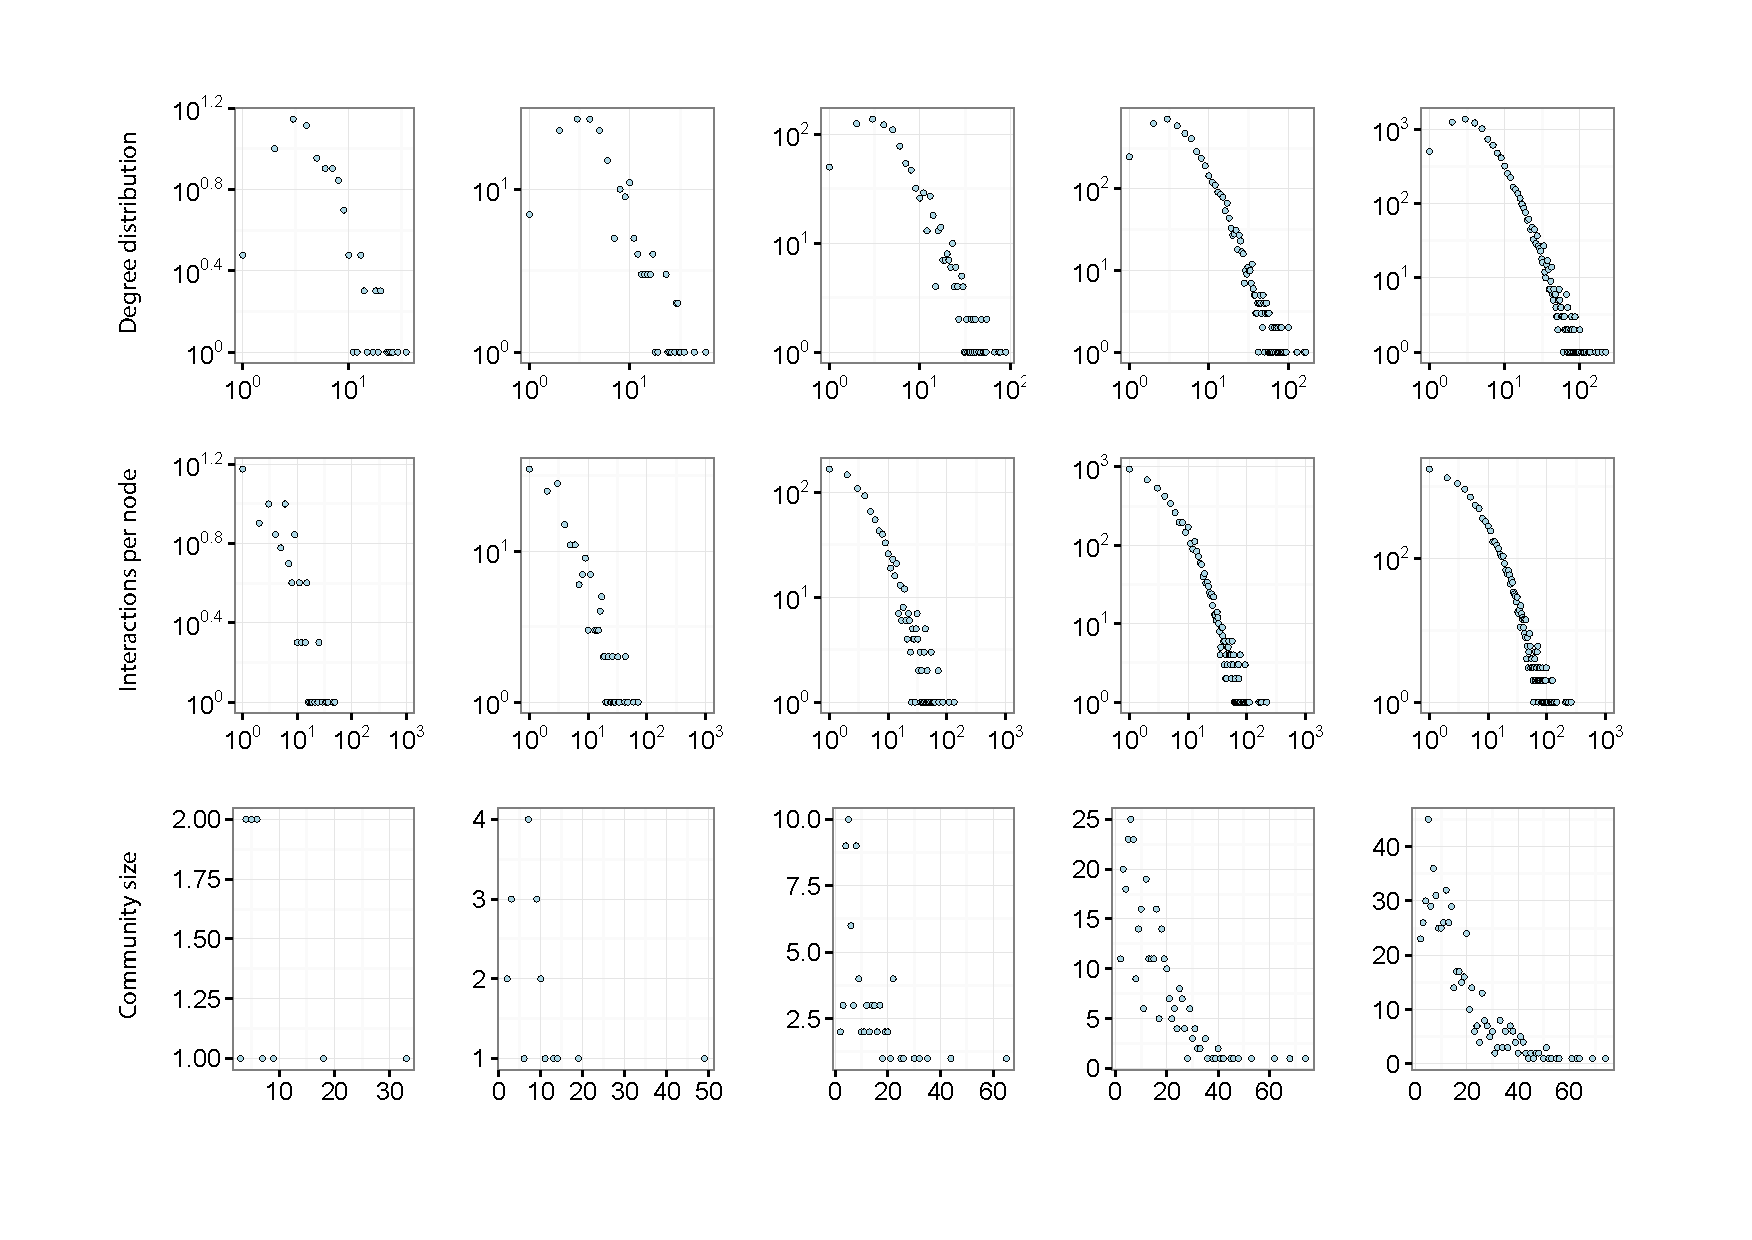
\includegraphics[width=46em]{figures/distribution_10_20_50}
\caption{Evolution of network (100, 200, 1000, 5000, 10000 nodes)}
\label{fig:EvolNet}
\end{figure*}

Key properties (average degree, shortest path, clustering coefficient, assortativity, modularity) happen to stabilize their values between $1000$ and $10000$ nodes. Our experiments show that  generated networks with other settings also have similar behavior. Figure \ref{fig:InterEvol} shows the evolution of the number of interactions for fifteen nodes with the highest number of interactions at the end of the generation process. The ID of a node represents the moment of its creation. The trend shows how the chances of participating in interactions increase for nodes that already have a high number of interactions.

\begin{figure}[ht]
\centering
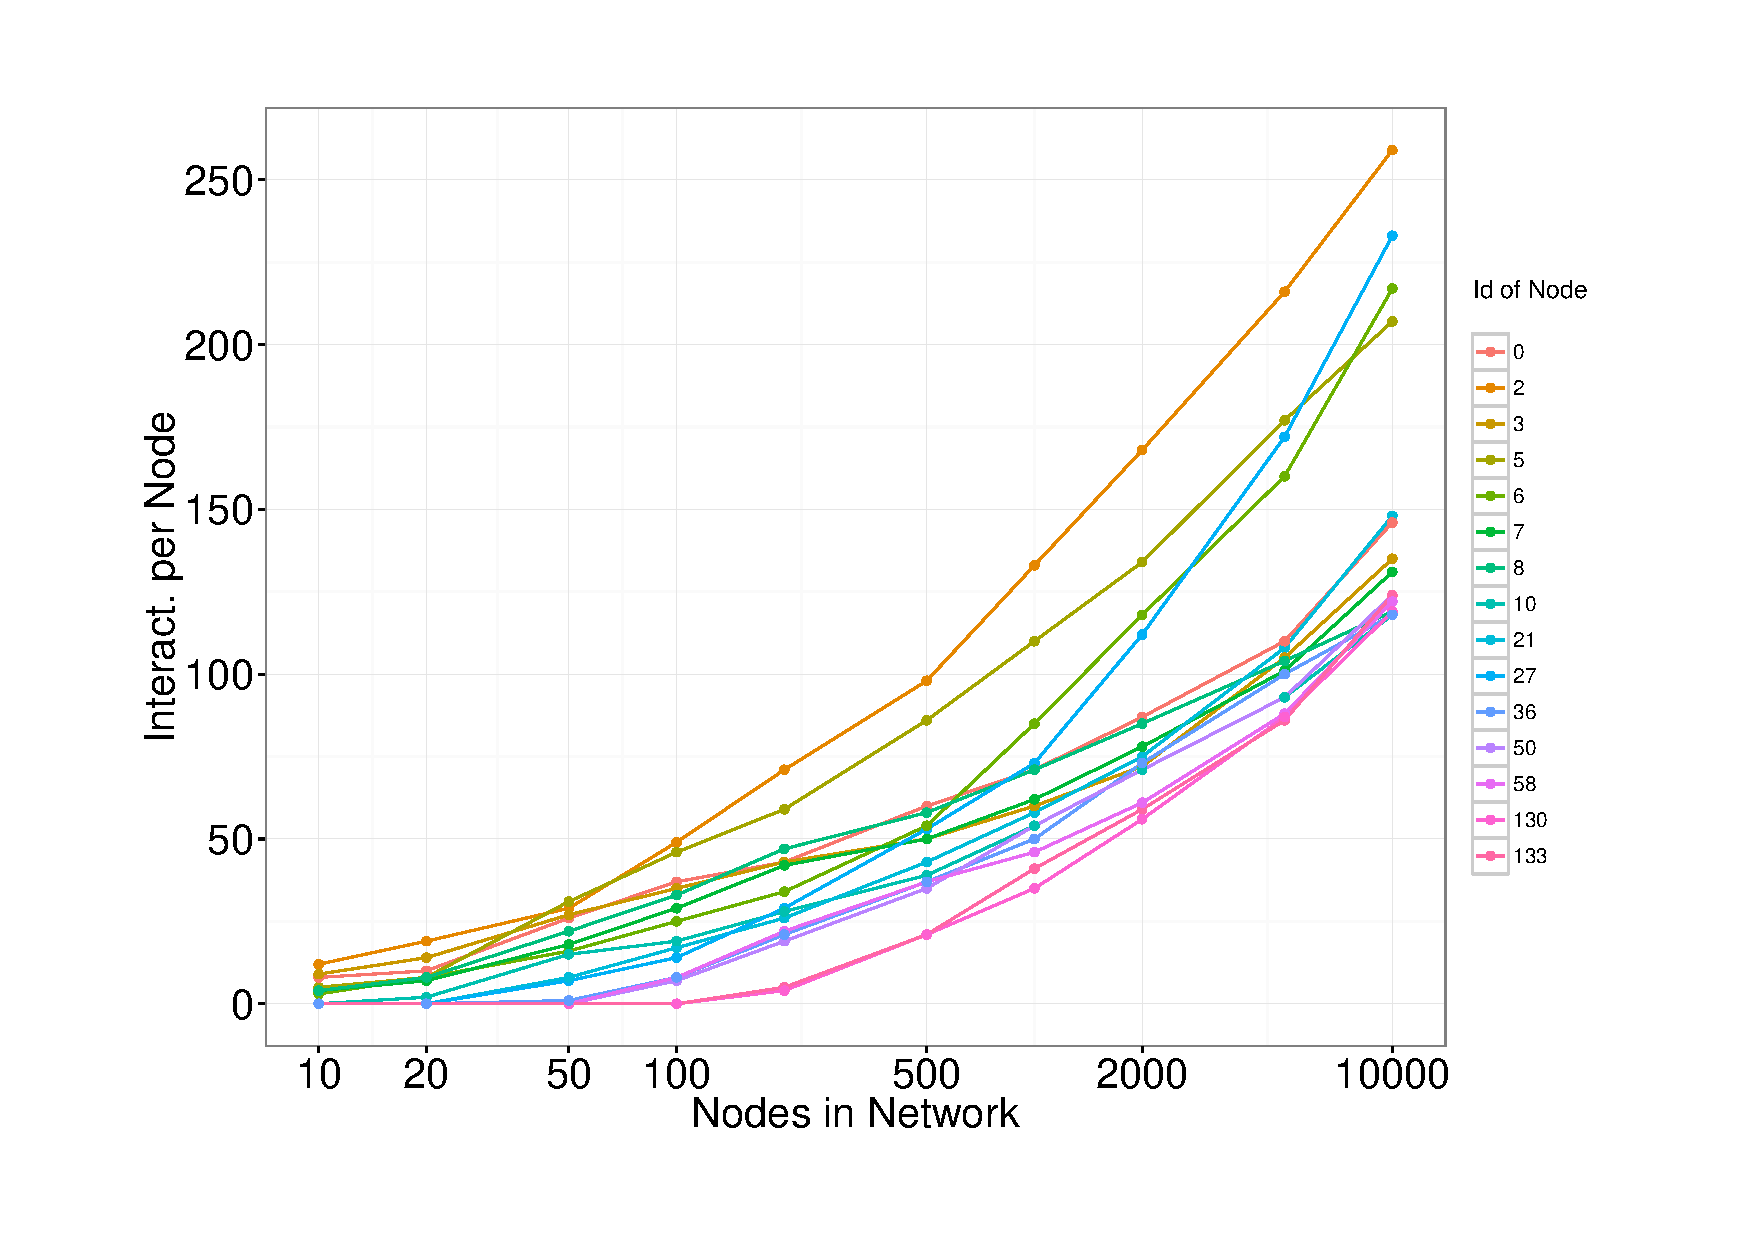
\includegraphics[width =\linewidth]{figures/Interaction_evolution}
\caption{Evolution of nodes with the most interactions}
\label{fig:InterEvol}
\end{figure}


\subsection{Correlations}
In this experiment, we compare the analyzed real-world network with generated networks. For each setting we generated a network with one million nodes. Then we examined the correlation between the node's creation time and it's degree and number of interactions, respectively. The emergence of the node is represented by its $ID$, which is in the order of its creation. Furthermore, we calculated the correlation between degree and number of node's interactions. We did the same for the analyzed DBLP dataset, where the order of nodes is to be understood as an estimate based on data pre-processing described in Section \ref{sec:dblp}.

\begin{table}[ht]
  \centering
  \caption{Correlations}
\begin{tabular}{|r|rrr|}
	\hline
Setting & $\rho(Id, k)$ & $\rho(Id, i)$ & $\rho(k, i)$ \\ 
\hline
$Setting_1$ & -0.59 & -0.50 & 0.96 \\  
\hline	
$Setting_2$ & -0.47 & -0.47 & 0.95 \\ 
\hline	
$Setting_3$ & -0.70 & -0.58 & 0.87 \\ 
\hline
DBLP & -0.23 & -0.18 & 0.84 \\ 
\hline
	\end{tabular}%
  \label{tab:corr}%
\end{table}%

The results summarized in Table \ref{tab:corr} show that regardless of the setting, the first two correlations are much higher in the 3-lambda model than in the DBLP dataset (Pearson's correlation coefficient was used). Thus, in the presented model, older nodes have a higher (and continuous) chance to participate in interactions than in reality. The cause is probably the aging of nodes in real-world networks where nodes, at different times, no longer participate in interactions. This significantly affects the evolution (growth) and some properties of the network.

Previous experiments demonstrated that despite the absence of aging, generated networks have very good properties. We have not, therefore, for reasons of simplicity, incorporated any of the known models of aging (e.g. inspired by \cite{dorogovtsev2000evolution, xu2010evolutionary}) to the 3-lambda network model.

\section{Conclusion}
\label{sec:conc}
Evolution of real-world networks is influenced by many factors. The purpose of network models is to discover these factors and describe them in a simple way. Our research focused on analyzing behavioral patterns of nodes existing in a co-authorship network while participating in publishing activities. We described four roles of nodes involved in interactions. Based on the analysis of the DBLP dataset, we formulated the hypothesis, which assumes that the numbers of nodes involved in interactions revolve around an average, and they are independent Poisson variables. Based on this hypothesis, we defined the 3-lambda model of collaborative network. The model has three parameters and has no memory. In three experiments, based on three different settings corresponding to dyads, triads and larger groups behavior, we showed that networks generated by the 3-lambda model have the characteristics known from the environment of real-world social networks. Furthermore, we showed that the model can be understood as temporal. In one experiment we presented the development and stabilization of generated network properties in time. For future research there remain some open questions. They bear relation to recognizing other factors influencing the development of the network and to the detailed study of the dependence and predictability of properties of generated networks on the setting of three network parameters (lambdas).

%ACKNOWLEDGMENTS are optional
\section{Acknowledgments}
This work was supported by SGS, VSB-Technical University of Ostrava, under the grant ``Parallel Processing of Big Data'', no. SP2016/97.

% The following two commands are all you need in the
% initial runs of your .tex file to
% produce the bibliography for the citations in your paper.
\bibliographystyle{abbrv}
\bibliography{references}  % sigproc.bib is the name of the Bibliography in this case
% You must have a proper ".bib" file
%  and remember to run:
% latex bibtex latex latex
% to resolve all references
%
% ACM needs 'a single self-contained file'!

\balancecolumns % GM June 2007
% That's all folks!
\end{document}


